\input format.tex

\begin{document}

\setlength{\arrayrulewidth}{1pt}
\fontsize{9.3pt}{17pt}\selectfont
\color{gray2}

\vspace*{0mm}

\begin{center}
{\bf\sanhao 检测结果}
\end{center}

\medskip
\noindent
{\liuhao 质地:~
\includegraphics[scale=0.6]{texture_part4.pdf}  ~~颜色:~
\includegraphics[scale=0.7]{color_part4.pdf}}
%{\liuhao 质地:无\hspace*{2cm} 颜色:无}
\hfill {\liuhao |~~颜色指示: \tikz\draw[green2,fill=green2](0,0) circle[radius=3.5pt]; 绿色为正常 \tikz\draw[yellow,fill=yellow](0,0) circle[radius=3.5pt]; 橙色为需要关注 \tikz\draw[red,fill=red](0,0) circle[radius=3.5pt]; 红色为有风险}

\medskip
\noindent
\begin{minipage}[b]{.24\textwidth}
\fontsize{9.3pt}{10pt}\selectfont
\medskip
\begin{tctabularx}{tabularx={p{3.33cm}}}
\parbox[c]{\hsize}{\vskip4pt{\color{black70} 消化和吸收\par \barial{INSUFFICIENCY}}\vskip4pt}\\\\[-5pt]
\begin{minipage}[t][1.6cm][t]{3.33cm}
\color{black70}
{\qihao 脂肪总量  \triangleb }\\
{\qihao 甘油三酯代谢  \triangleb }\\
{\qihao 甘油磷脂代谢  \triangleb }\\
{\qihao ~}\\
\end{minipage}
\\[-5pt]
\centerline{
\includegraphics[width=2.15cm]{INSUFFICIENCY-yellow.pdf}}\\[-5pt]
\hspace*{0cm}\begin{minipage}[t][1.2cm][t]{3cm}{
%
\includegraphics{diandian.pdf}
\tikz\draw[topcolor,fill=topcolor](0,0) circle[radius=1pt];
\color{gray2}\qihao
%您的脂肪总量、甘油三酯代谢、甘油磷脂代谢指标异常。
您的消化吸收检测出3项异常指标。
}\end{minipage}\\
\centerline{\color{gray2}\rule{3cm}{0.5pt}}\\[-5pt]
\bahao
\noindent\begin{tabular}{@{}m{0.83cm}<{\centering}@{}m{0.83cm}<{\centering}@{}m{0.83cm}<{\centering}@{}m{0.83cm}<{\centering}@{}}

\includegraphics[width=.45cm]{sun-yellow.pdf} & \tikz\draw[gray,fill=gray](0,0) circle[radius=4.5pt]; & \tikz\draw[gray,fill=gray](0,0) circle[radius=4.5pt]; & \tikz\draw[gray,fill=gray](0,0) circle[radius=4.5pt];\\
\color{gray2}当次 & \color{gray2} & \color{gray2} & \color{gray2}
\\
\end{tabular}
\end{tctabularx}
\end{minipage}
\hfill
\noindent
\begin{minipage}[b]{.24\textwidth}
\fontsize{9.3pt}{10pt}\selectfont
\medskip
\begin{tctabularx}{tabularx={p{3.33cm}}}
\parbox[c]{\hsize}{\vskip4pt{\color{black70} 炎症和免疫\par \barial{INFLAMMATION}}\vskip4pt}\\\\[-5pt]
\begin{minipage}[t][1.6cm][t]{3.33cm}
\color{black70}
{\qihao 免疫指数  \triangleb }\\
{\qihao ~}\\
{\qihao ~}\\
{\qihao ~}\\
\end{minipage}
\\[-5pt]
\centerline{
\includegraphics[width=2.15cm]{INFLAMMATION-yellow.pdf}}\\[-5pt]
\hspace*{0cm}\begin{minipage}[t][1.2cm][t]{3.3cm}{
\tikz\draw[topcolor,fill=topcolor](0,0) circle[radius=1pt];
\color{gray2}\qihao
您的免疫指数指标异常。
}\end{minipage}\\
\centerline{\color{gray2}\rule{3cm}{0.5pt}}\\[-5pt]
\bahao
\noindent\begin{tabular}{@{}m{0.83cm}<{\centering}@{}m{0.83cm}<{\centering}@{}m{0.83cm}<{\centering}@{}m{0.83cm}<{\centering}@{}}

\includegraphics[width=.45cm]{sun-yellow.pdf} & \tikz\draw[gray,fill=gray](0,0) circle[radius=4.5pt]; & \tikz\draw[gray,fill=gray](0,0) circle[radius=4.5pt]; & \tikz\draw[gray,fill=gray](0,0) circle[radius=4.5pt];\\
\color{gray2}当次 & \color{gray2} & \color{gray2} & \color{gray2}
\\
\end{tabular}
\end{tctabularx}
\end{minipage}
\hfill
\noindent
\begin{minipage}[b]{.24\textwidth}
\fontsize{9.3pt}{10pt}\selectfont
\medskip
\begin{tctabularx}{tabularx={p{3.33cm}}}
\parbox[c]{\hsize}{\vskip4pt{\color{black70} 致病菌\par \barial{INFECTION}}\vskip4pt}\\\\[-5pt]
\begin{minipage}[t][1.6cm][t]{3.33cm}
\color{black70}
{\qihao 脆弱拟杆菌 }\\
{\qihao ~}\\
{\qihao ~}\\
{\qihao ~}\\
\end{minipage}
\\[-5pt]
\centerline{
\includegraphics[width=2.15cm]{INFECTION-yellow.pdf}}\\[-5pt]
\hspace*{0cm}\begin{minipage}[t][1.2cm][t]{3.3cm}{
\tikz\draw[topcolor,fill=topcolor](0,0) circle[radius=1pt];
\color{gray2}\qihao
您的肠道中检测出1种致病菌,含量未超标。
}\end{minipage}\\
\centerline{\color{gray2}\rule{3cm}{0.5pt}}\\[-5pt]
\bahao
\noindent\begin{tabular}{@{}m{0.83cm}<{\centering}@{}m{0.83cm}<{\centering}@{}m{0.83cm}<{\centering}@{}m{0.83cm}<{\centering}@{}}

\includegraphics[width=.45cm]{sun-yellow.pdf} & \tikz\draw[gray,fill=gray](0,0) circle[radius=4.5pt]; & \tikz\draw[gray,fill=gray](0,0) circle[radius=4.5pt]; & \tikz\draw[gray,fill=gray](0,0) circle[radius=4.5pt];\\
\color{gray2}当次 & \color{gray2} & \color{gray2} & \color{gray2}
\\
\end{tabular}
\end{tctabularx}
\end{minipage}
\hfill
\noindent
\begin{minipage}[b]{.24\textwidth}
\fontsize{9.3pt}{10pt}\selectfont
\medskip
\begin{tctabularx}{tabularx={p{3.33cm}}}
\parbox[c]{\hsize}{\vskip4pt{\color{black70} 代谢平衡\par \barial{IMBALANCE}}\vskip4pt}\\\\[-5pt]
\begin{minipage}[t][1.6cm][t]{3.33cm}
\color{black70}
{\qihao 胆碱  \trianglea }\\
{\qihao ~}\\
{\qihao ~}\\
{\qihao ~}\\
\end{minipage}
\\[-5pt]
\centerline{
\includegraphics[width=2.15cm]{IMBALANCE-yellow.pdf}}\\[-5pt]
\hspace*{0cm}\begin{minipage}[t][1.2cm][t]{3.3cm}{
\tikz\draw[topcolor,fill=topcolor](0,0) circle[radius=1pt];
\color{gray2}\qihao
%您的胆碱指标异常。
您的重要小分子代谢检测出1项异常指标。
}\end{minipage}\\
\centerline{\color{gray2}\rule{3cm}{0.5pt}}\\[-5pt]
\bahao
\noindent\begin{tabular}{@{}m{0.83cm}<{\centering}@{}m{0.83cm}<{\centering}@{}m{0.83cm}<{\centering}@{}m{0.83cm}<{\centering}@{}}

\includegraphics[width=.45cm]{sun-yellow.pdf} & \tikz\draw[gray,fill=gray](0,0) circle[radius=4.5pt]; & \tikz\draw[gray,fill=gray](0,0) circle[radius=4.5pt]; & \tikz\draw[gray,fill=gray](0,0) circle[radius=4.5pt];\\
\color{gray2}当次 & \color{gray2} & \color{gray2} & \color{gray2}
\\
\end{tabular}
\end{tctabularx}
\end{minipage}

\vspace*{-4mm}
%\medskip
\noindent
\begin{minipage}[t][8cm][t]{.35\textwidth}
\fontsize{9.3pt}{10pt}\selectfont
\medskip
\begin{tctabularx}{tabularx={p{5.06cm}}}
\parbox[c]{\hsize}{\vskip4pt{\color{black70} 菌群多样性\par \barial{DIVERSITY ASSOCIATION}}\vskip4pt}\\
\parbox[c]{\hsize}{\vskip4pt{\tikz\draw[topcolor,fill=topcolor](0,0) circle[radius=1pt];\color{gray2}\qihao 您的菌群多样性仅高于6.10{\%}的参考人群}\\}
\parbox[c]{\hsize}{
\begin{center}
\begin{picture}(1, 1)
\put(-70, -165){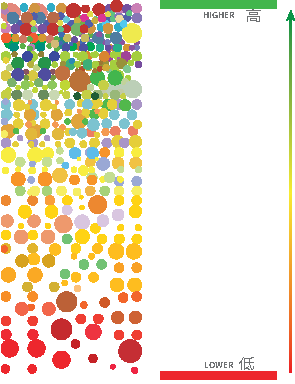
\includegraphics[width=4.70cm]{DIVERSITY-ASSOCIATION.pdf}}
\put(3, -146){\raisebox{6.10pt}{
\includegraphics[scale=0.85]{DIVERSITY-low.pdf}}}
\end{picture}
\end{center}
}
\\\\\\\\\\\\\\[-7pt]
\\\\\\\\\\\\\\
\\\\\\\\
\end{tctabularx}
\end{minipage}
\hfill
\begin{minipage}[t][8cm][t]{.637\textwidth}
\fontsize{9.3pt}{10pt}\selectfont
\medskip
\begin{tctabularx}{tabularx={p{9.59cm}}}
\parbox[c]{\hsize}{\vskip4pt{\color{black70} 相对丰度\par \barial{RELATIVE ABUNDANCE}}\vskip4pt}\\\\
%\begin{center}

\hspace*{0.2cm}
{
\begin{tikzpicture}[bar interval width=0.8, bar width=0.70cm]
	\draw[black]
		(-3cm, 0.0cm) node[left, anchor = west] {\color{black70} {正常人的结果}}
		(-3cm, 1.0cm) node[left, anchor = west] {\color{black70} {您的结果}}
		;
	\begin{scope}
	\clip[] (0cm, -0.30cm) rectangle (5cm, 0.30cm);
	\draw[fill=solomon0, solomon0] (0cm * 5, -0.30cm) rectangle (0.4638738cm * 5, 0.30cm) node {};
	\draw[fill=solomon1, solomon1] (0.4638738cm * 5, -0.30cm) rectangle (0.53750432cm * 5, 0.30cm) node {};
	\draw[fill=solomon2, solomon2] (0.53750432cm * 5, -0.30cm) rectangle (0.96469122cm * 5, 0.30cm) node {};
	\draw[fill=solomon3, solomon3] (0.96469122cm * 5, -0.30cm) rectangle (0.97686611cm * 5, 0.30cm) node {};
	\draw[fill=solomon4, solomon4] (0.97686611cm * 5, -0.30cm) rectangle (0.9768664906821cm * 5, 0.30cm) node {};
	\draw[fill=solomon5, solomon5] (0.9768664906821cm * 5, -0.30cm) rectangle (0.9768761320951cm * 5, 0.30cm) node {};
	\draw[fill=solomon6, solomon6] (0.9768761320951cm * 5, -0.30cm) rectangle (0.9957773020951cm * 5, 0.30cm) node {};
%	\draw[fill=green, green] (0cm, -0.30cm) rectangle (1cm, 0.30cm) node {};%[xshift = -0.966091954022989cm,yshift=-4.5mm];
%	\draw[fill=red, red] (1cm, -0.30cm) rectangle (4cm, 0.30cm) node {};%[xshift = -1.08390804597701cm,yshift=-4.5mm];
%	\draw[fill=blue, blue] (4cm, -0.30cm) rectangle (5cm, 0.30cm) node {};%[xshift = -0.45cm,yshift=-4.5mm];
	\end{scope}
	\begin{scope}
	\clip[] (0cm, 0.70cm) rectangle (5cm, 1.30cm);
	\draw[fill=solomon0, solomon0] (0cm * 5, 0.70cm) rectangle (0.9316207cm * 5, 1.30cm) node {};
	\draw[fill=solomon1, solomon1] (0.9316207cm * 5, 0.70cm) rectangle (0.97271659cm * 5, 1.30cm) node {};
	\draw[fill=solomon2, solomon2] (0.97271659cm * 5, 0.70cm) rectangle (0.99836832cm * 5, 1.30cm) node {};
	\draw[fill=solomon3, solomon3] (0.99836832cm * 5, 0.70cm) rectangle (0.99840626634cm * 5, 1.30cm) node {};
	\draw[fill=solomon4, solomon4] (0.99840626634cm * 5, 0.70cm) rectangle (0.99840626634cm * 5, 1.30cm) node {};
	\draw[fill=solomon5, solomon5] (0.99840626634cm * 5, 0.70cm) rectangle (0.99840626634cm * 5, 1.30cm) node {};
	\draw[fill=solomon6, solomon6] (0.99840626634cm * 5, 0.70cm) rectangle (0.99840626634cm * 5, 1.30cm) node {};
%	\draw[fill=green,green] (0cm, 0.70cm) rectangle (1.30cm, 1.30cm) node {};%[xshift = -0.966091954022989cm,yshift=-4.5mm];
%	\draw[fill=red,red] (1.30cm, 0.70cm) rectangle (3.5cm, 1.30cm) node {};%[xshift = -1.08390804597701cm,yshift=-4.5mm];
%	\draw[fill=blue, blue] (3.5cm, 0.70cm) rectangle (5cm, 1.30cm) node {};%[xshift = -0.30cm,yshift=-4.5mm];
	\end{scope}

	\draw[fill=solomon0, solomon0](-2.8cm, -2.20cm - 0.40cm * 0) rectangle (-2cm, -2.0cm - 0.40cm * 0);
	\draw (-2cm, -2.20cm - 0.40cm * 0) node[left, anchor = west, yshift=1.2mm] {\wudianwu\color{gray2} {Bacteroidetes~~拟杆菌门}};
	\draw[fill=solomon1, solomon1](-2.8cm, -2.20cm - 0.40cm * 1) rectangle (-2cm, -2.0cm - 0.40cm * 1);
	\draw (-2cm, -2.20cm - 0.40cm * 1) node[left, anchor = west, yshift=1.2mm] {\wudianwu\color{gray2} {Proteobacteria~~变形菌门}};
	\draw[fill=solomon2, solomon2](-2.8cm, -2.20cm - 0.40cm * 2) rectangle (-2cm, -2.0cm - 0.40cm * 2);
	\draw (-2cm, -2.20cm - 0.40cm * 2) node[left, anchor = west, yshift=1.2mm] {\wudianwu\color{gray2} {Firmicutes~~厚壁菌门}};
	\draw[fill=solomon3, solomon3](-2.8cm, -2.20cm - 0.40cm * 3) rectangle (-2cm, -2.0cm - 0.40cm * 3);
	\draw (-2cm, -2.20cm - 0.40cm * 3) node[left, anchor = west, yshift=1.2mm] {\wudianwu\color{gray2} {Actinobacteria~~放线菌门}};
	\draw[fill=solomon4, solomon4](-2.8cm, -2.20cm - 0.40cm * 4) rectangle (-2cm, -2.0cm - 0.40cm * 4);
	\draw (-2cm, -2.20cm - 0.40cm * 4) node[left, anchor = west, yshift=1.2mm] {\wudianwu\color{gray2} {Spirochaetes~~螺旋体门}};
	\draw[fill=solomon5, solomon5](-2.8cm, -2.20cm - 0.40cm * 5) rectangle (-2cm, -2.0cm - 0.40cm * 5);
	\draw (-2cm, -2.20cm - 0.40cm * 5) node[left, anchor = west, yshift=1.2mm] {\wudianwu\color{gray2} {Armatimonadetes~~装甲菌门}};
	\draw[fill=solomon6, solomon6](-2.8cm, -2.20cm - 0.40cm * 6) rectangle (-2cm, -2.0cm - 0.40cm * 6);
	\draw (-2cm, -2.20cm - 0.40cm * 6) node[left, anchor = west, yshift=1.2mm] {\wudianwu\color{gray2} {Fusobacteria~~梭杆菌门}};
	\draw[fill=gray2, gray2](-3.00cm, -1.80cm) node[left, anchor = west, yshift=1.2mm] {\wudianwu\color{black} {细菌门水平分类}};

	\draw (1.5cm, -3.3cm) node[right, anchor = west, yshift=1.2mm] {\xiaosihao\color{gray2} {您的菌群相对丰度与}};
		\draw (1.5cm, -3.9cm) node[right, anchor = west, yshift=1.2mm] {\xiaosihao\color{gray2} {参考人群趋势差异较大}};
	%	\draw[fill=blue, blue](-2.8cm, -5.00cm + 0.40cm * 0) rectangle (-2cm, -4.8cm + 0.40cm * 0); \draw (-2cm, -5.00cm + 0.40cm * 0) node[left, anchor = west, yshift=1.2mm] {\wudianwu {xxx 所罗门}};
%	\draw[fill=blue, blue](-2.8cm, -5.00cm + 0.40cm * 1) rectangle (-2cm, -4.8cm + 0.40cm * 1); \draw (-2cm, -5.00cm + 0.40cm * 1) node[left, anchor = west, yshift=1.2mm] {\wudianwu {xxx 所罗门}};
%	\draw[fill=blue, blue](-2.8cm, -5.00cm + 0.40cm * 2) rectangle (-2cm, -4.8cm + 0.40cm * 2); \draw (-2cm, -5.00cm + 0.40cm * 2) node[left, anchor = west, yshift=1.2mm] {\wudianwu {xxx 所罗门}};
%	\draw[fill=blue, blue](-2.8cm, -5.00cm + 0.40cm * 3) rectangle (-2cm, -4.8cm + 0.40cm * 3); \draw (-2cm, -5.00cm + 0.40cm * 3) node[left, anchor = west, yshift=1.2mm] {\wudianwu {xxx 所罗门}};
%	\draw[fill=blue, blue](-2.8cm, -5.00cm + 0.40cm * 4) rectangle (-2cm, -4.8cm + 0.40cm * 4); \draw (-2cm, -5.00cm + 0.40cm * 4) node[left, anchor = west, yshift=1.2mm] {\wudianwu {xxx 所罗门}};
%	\draw[fill=blue, blue](-2.8cm, -5.00cm + 0.40cm * 5) rectangle (-2cm, -4.8cm + 0.40cm * 5); \draw (-2cm, -5.00cm + 0.40cm * 5) node[left, anchor = west, yshift=1.2mm] {\wudianwu {xxx 所罗门}};
%	\draw[fill=blue, blue](-2.8cm, -5.00cm + 0.40cm * 6) rectangle (-2cm, -4.8cm + 0.40cm * 6); \draw (-2cm, -5.00cm + 0.40cm * 6) node[left, anchor = west, yshift=1.2mm] {\wudianwu {xxx 所罗门}};

%	\draw[fill=black, black](-2.0cm, -5.00cm + 0.40cm * 7) node[left, anchor = west, yshift=1.2mm] {\wudianwu\color{black} {xxx 所罗门}};


\end{tikzpicture}
}

%\end{center}
\end{tctabularx}
\end{minipage}

\vfill

\end{document}

